\documentclass{article} % For LaTeX2e
\usepackage{nips15submit_e,times}
\usepackage{hyperref}
\usepackage{url}
\usepackage{graphicx}
\usepackage{amsfonts}
\usepackage{amssymb}
\usepackage{float}
\usepackage{listings}
\usepackage{xcolor}
\usepackage{amsmath}
%\documentstyle[nips14submit_09,times,art10]{article} % For LaTeX 2.09


\title{Problem Set 3 for Machine Learning 15 Fall}


\author{
Jingyuan Liu\\
AndrewId: jingyual\\
\texttt{jingyual@andrew.cmu.edu} \\
}


\newcommand{\fix}{\marginpar{FIX}}
\newcommand{\new}{\marginpar{NEW}}
\newcommand{\argmin}{\arg\!\min}
\newcommand{\norm}[1]{\left\lVert #1 \right\rVert}
\newcommand{\abs}[1]{\left\lvert #1 \right\rvert}
\newcommand{\inner}[1]{\left\langle #1 \right\rangle}


\nipsfinalcopy % Uncomment for camera-ready version


\begin{document}
\maketitle



\section{Neural Networks}


For convenience, we can denote the nodes in the first layer as $n_1, n_2$, the
second layer $n_3$.

\subsection{Neural network for regression}
\textbf{1.1.1. Simulating linear regression}

In this scenario, every node should use S.

\begin{equation}
n_1 = c(x_1 w_1 + x_2 w_3), \quad
n_2 = c(x_1 w_2 + x_2 w_4)
\end{equation}

\begin{equation}
y = c n_3 =  c(n_1 w_5 + n_2 w_6)
\end{equation}

\begin{equation}
\qquad \qquad \qquad \qquad \quad
= c^2 ((x_1 w_1 + x_2 w_3) w_5 + (x_1 w_2 + x_2 w_4) w_6)
\end{equation}

\begin{equation}
\qquad \qquad \qquad \qquad \quad
= c^2 (w_1 w_5 + w_2 w_6) x_1 + c^2 (w_3 w_5 + w_4 w_6) x_2
\end{equation}

\begin{equation}
\beta_1 = c^2 (w_1 w_5 + w_2 w_6),  \quad
\beta_2 = c^2 (w_3 w_5 + w_4 w_6)
\end{equation}

\textbf{1.1.2. Derive $\beta_1$ and $\beta_2$}

In this scenario, $n_1$ and $n_2$ should use L, and $n_3$ should use S.

\begin{equation}
n_1 = c(x_1 w_1 + x_2 w_3), \quad
n_2 = c(x_1 w_2 + x_2 w_4)
\end{equation}

\begin{equation}
p(n_3 = 1 \mid X) = \frac{1}{1 + exp(-(n_1 w_5 + n_2 w_6))}
\end{equation}

\begin{equation}
\qquad \qquad \quad = \frac{exp(n_1 w_5 + n_2 w_6)}{1 + exp(n_1 w_5 + n_2 w_6)}
\end{equation}

According to the defination of S, we know that the Y = 1 when $n_3$ = 1, and Y = -1
when $n_3$ = 0. Therefore, we can derive that:

\begin{equation}
P(Y=1 \mid X) = p(n_3 = 1 \mid X) = \frac{exp(n_1 w_5 + n_2 w_6)}
{1 + exp(n_1 w_5 + n_2 w_6)}
\end{equation}

\begin{equation}
\beta_1 = c (w_1 w_5 + w_2 w_6),  \quad
\beta_2 = c (w_3 w_5 + w_4 w_6)
\end{equation}

\textbf{1.1.3. Derive $\alpha_1$ and $\alpha_2$}

In this scenario, $n_1$ and $n_2$ should use S, and $n_3$ should use L. For f1
and f2, they employ the same distribution as 1.1.2, so:

\begin{equation}
p(Y_1=1 \mid X, f1) = p (n_1=1 \mid x)
= \frac{exp(w_1 x_1 + w_3 x_2)}{1 + exp(w_1 x_1 + w_3 x_2)}
\end{equation}

\begin{equation}
p(Y_2=1 \mid X, f2) = p (n_2=1 \mid x)
= \frac{exp(w_2 x_1 + w_4 x_2)}{1 + exp(w_2 x_1 + w_4 x_2)}
\end{equation}

For $n_3$ and Y, we have:

\begin{equation}
n_3 = n_1 w_5 + n_2 w_6, \quad
y = c n_3 = sign(\alpha_1 Y_1 + \alpha_2 Y_2)
\end{equation}

\begin{equation}
\alpha_1 = c w_5, \quad
\alpha_2 = c w_6
\end{equation}


\subsection{Convolutional Neural Networks}


\subsection{Gradient vanishing/explosion}

\textbf{1.3.1 Derive b1, the first layer bias}

We can derive the derivative of L w.r.t. b1 using the chain rule:

\begin{equation}
\frac{\partial L}{\partial b_1} =
\frac{\partial L}{\partial z_m} \frac{\partial z_m}{\partial z_{m-1}} ...
\frac{\partial z_{2}}{\partial z_{1}} \frac{\partial z_{1}}{\partial b_1}
\end{equation}

\begin{equation}
\qquad \qquad \qquad
= \frac{\partial L}{\partial z_m}
\cdot \sigma' (w_1 x + b_1)
\cdot \prod_{k=1}^m \frac{\partial z_{k+1}}{\partial z_k}
\end{equation}

\textbf{1.3.2. (a) explain vanish trend}

As the activation function is given, we can derive:

\begin{equation}
\frac{\partial z_{k+1}}{\partial z_k} =
\frac{\partial \sigma (w_k z_k + b_k)}{\partial (w_k z_k + b_k)}
\cdot \frac{\partial (w_k z_k + b_k)}{\partial z_k}
\end{equation}

\begin{equation}
\qquad \qquad \qquad =
\sigma (w_k z_k + b_k) (1- \sigma (w_k z_k + b_k))
\cdot w_k
\end{equation}

As we know, $\sigma (x)$ and $1-\sigma (x)$ is smaller than 1, and $\abs{w_k}$
is smaller than 1. Therefore, according what we derived from 1.3.1, we would
konw that the $\frac{\partial L}{\partial b_1}$ tends to vanish when m is large.

\textbf{1.3.2. (b) explain vanish trend given large $\abs{w}$}

Given the form of the $\frac{\partial z_{k+1}}{\partial z_k}$, we can simple
consider this function:

\begin{equation}
f_{temp} = \frac{x \cdot exp(x)}{ (1+exp(x))^2}
\end{equation}

which is the same ``form'' of the derivative. As we can see, with increase of x,
the $f_{temp}$ would become smaller and would be smaller than 1. The trend of
$\frac{\partial z_{k+1}}{\partial z_k}$ is the same. When the $\abs{w}$ is
large, the total $\frac{\partial z_{k+1}}{\partial z_k}$ would still be smaller
than 1, because the decreasing trend of
$\sigma (w_k z_k + b_k) (1- \sigma (w_k z_k + b_k))$ would be more influential
than the increasing trend of $w_k$.

\textbf{1.3.2. (b) explain vanish trend given large $\abs{w}$}


\textbf{1.3.3. Explain the ReL}


\textbf{1.3.4. Prove the equation}

From the equation, we can derive:

\begin{equation}
\frac{\partial log p(v)}{\partial \theta_i} =
\frac{\partial log \sum_h p(v, h)}{\partial \theta_i}
\end{equation}

\begin{equation}
log \sum_h p(v,h) = log \sum_h exp(\sum_i \theta_i \phi_i (v,h))
- log (\sum_{v,h} exp (\sum_i \theta_i \phi_i (v,h)))
\end{equation}

For simplicity, we can use $\phi_i$ to replace $\phi_i (v,h)$,
the first part and second part:

\begin{equation}
\frac{\partial log \sum_h p(v,h)}{\partial \theta_i} =
\frac{1}{\sum_h exp(\sum_i \theta_i \phi_i)} \cdot
\frac{\partial \sum_h exp(\sum_i \theta_i \phi_i)}{\partial \theta_i} \cdot
\end{equation}

\begin{equation}
\qquad \qquad \qquad \quad =
\frac{1}{\sum_h exp(\sum_i \theta_i \phi_i)} \cdot
\sum_h exp(\sum_i \theta_i \phi_i) \cdot \phi_i
\end{equation}

\begin{equation}
= \sum_h \phi_i \frac{exp(\sum_i \theta_i \phi_i)}
{\sum_h exp(\sum_i \theta_i \phi_i)}
\end{equation}

Using bayes rule, we can derive the first part as:

\begin{equation}
p (h \mid v) = \frac{p(v,h)}{p(v)} = \frac{p(v,h)}{\sum_h p(v,h)}
\end{equation}

\begin{equation}
\qquad = 
\frac{exp(\sum_i \theta_i \phi_i)}{\sum_h exp(\sum_i \theta_i \phi_i)}
\end{equation}

\begin{equation}
\frac{\partial log \sum_h p(v,h)}{\partial \theta_i} =
\sum_h \phi(v,h) p (h \mid v)
\end{equation}

We can similarily derive the second part:

\begin{equation}
\frac{\partial \sum_{v,h} exp(\sum_i \theta_i \phi_i)}{\partial \theta_i}
= \frac{1}{Z} \cdot \frac{\partial \sum_{v,h} exp(\sum_i \theta_i \phi_i)}
{\partial \theta_i}
\end{equation}

\begin{equation}
\qquad \qquad \qquad \quad = 
\sum_{v,h} \phi_i \frac{exp(\sum_i \theta_i \phi_i)}{Z} 
\end{equation}

\begin{equation}
\qquad \qquad = 
\sum_{v,h} \phi_i p(v,h)
\end{equation}

Combine the two parts, we can get the conclusion:

\begin{equation}
\frac{\partial log p(v)}{\partial \theta_i} = \sum_h \phi_i (v,h) p(h \mid v)
- \sum_{v,h} \phi_i (v,h) p(v,h)
\end{equation}



\section{Regularized Linear Regression Using Lasso}

The visualization is as follows:

\begin{figure}[h]
\begin{center}
\label{fig:nn}
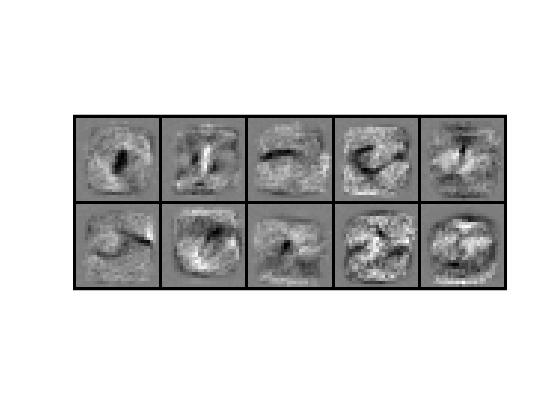
\includegraphics[width=12cm]{pic/result.jpg}
\caption{visualization}
\end{center}
\end{figure}



\section{Collaboration}
I dicussed with Zheng Chen with problem 2 on understanding finding the minimal
for a quardratic function. And discussed with him on question 4 about using the
cos value. And double checked the question 5 implementation.

\end{document}
